\documentclass[12pt]{amsart}
\hoffset=-.90in
\textwidth=6.5in
\voffset=-.5in
\textheight=9.0in
\setlength{\parindent}{0pt}

\makeindex
\usepackage{amssymb,amsmath,amsthm}
\usepackage[all]{xy}
\usepackage{enumerate}
\usepackage{tikz}
\usetikzlibrary{calc}

\renewcommand{\1}{^{-1}}
\renewcommand{\bar}{\overline}
\newcommand{\C}{\mathbb{C}}
\newcommand{\D}{\mathbb{D}}
\newcommand{\R}{\mathbb{R}}
\newcommand{\rank}{\hbox{\rm rank}}
\renewcommand{\S}{\mathbb{S}}
\renewcommand{\setminus}{\smallsetminus}
\newcommand{\SL}{\hbox{\rm SL}} % special linear group
\newcommand{\SO}{\hbox{\rm SO}} % special orthogonal group
\newcommand{\Supp}{\hbox{\rm Supp}} % support
\newcommand{\T}{\mathbb{T}}
\renewcommand{\tilde}{\widetilde}
\newcommand{\Z}{\mathbb{Z}}

\begin{document}

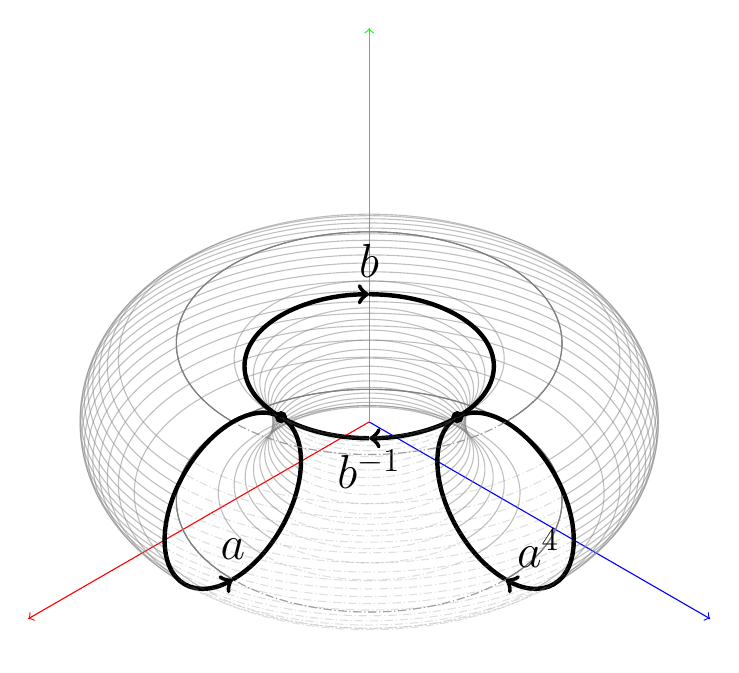
\begin{tikzpicture}
% the following is how i orient my 3d coordinate system, followed by colored axes
[x=(-150:1),y=(-135:sqrt(2)),z=(-135:sqrt(2))]
\coordinate (o) at (0,0,0);
\draw[->,color=red] (o)--(5,0,0);
\draw[->,color=blue] (o)--(0,5,0);
\draw[->,color=green] (o)--(0,0,5);
%
% to draw and fill the main torus,
\foreach \i in {-1,-0.9,...,0.9,1}{
\draw[color=gray,opacity=0.5*(1+(\i)^100)]
(${2+cos(asin(\i))}*(1,0,0)+(0,0,\i)$) arc (0:-270:{2+cos(asin(\i))}); % torus filling (outer)
%
\draw[color=gray,opacity=0.5*(1+(\i)^1000)]
(${2-cos(asin(\i))}*(1,0,0)+(0,0,\i)$) arc (0:-270:{2-cos(asin(\i))}); % torus filling (inner)
};
%
% base point and loops
\draw[fill] (${2-sqrt(2)/2}*(1,0,0)+sqrt(2)/2*(0,0,1)$) circle[radius=2pt];
\draw[fill] (${2-sqrt(2)/2}*(0,1,0)+sqrt(2)/2*(0,0,1)$) circle[radius=2pt];
\draw[ultra thick,->,z=(-135:sqrt(2)),y=(-135:sqrt(2))] ($sqrt(2)/2*(-1,1,0)+(2,0,0)$) arc (135:-90:1) node(a)[above=3pt]{\LARGE $a$}; 
\draw[ultra thick,z=(-135:sqrt(2)),y=(-135:sqrt(2))] (2,-1,0) arc (-90:-225:1); % generator a
\draw[ultra thick,->,line join=miter,y=(-135:sqrt(2)),x=(-135:sqrt(2))] ($sqrt(2)/2*(-1,1,0)+(2,0,0)$) arc (135:-90:1) node(a4)[above right]{\LARGE $a^4$};
\draw[ultra thick,y=(-135:sqrt(2)),x=(-135:sqrt(2))] (2,-1,0) arc (-90:-225:1); % generator a4
\draw[ultra thick,->] (${2-sqrt(2)/2}*(1,0,0)+sqrt(2)/2*(0,0,1)$) arc (0:-135:{2-sqrt(2)/2}) node(b)[above=2pt]{\LARGE $b$};
\draw[ultra thick] (${(sqrt(2)/2)*(2-sqrt(2)/2)}*(-1,-1,0)+sqrt(2)/2*(0,0,1)$) arc (-135:-270:{2-sqrt(2)/2}); % generator b
\draw[ultra thick,->] (${2-sqrt(2)/2}*(0,1,0)+sqrt(2)/2*(0,0,1)$) arc (90:45:{2-sqrt(2)/2}) node(binv)[below]{\LARGE $b\1$};
\draw[ultra thick] (${(sqrt(2)/2)*(2-sqrt(2)/2)}*(1,1,0)+sqrt(2)/2*(0,0,1)$) arc (45:0:{2-sqrt(2)/2}); % generator binv
%
% and attaching the last rectangle
\foreach \i in {-1,-0.9,...,0.9,1}{
\draw[densely dashdotted,color=gray,opacity=0.25*(1+(\i)^100)]
(${2+cos(asin(\i))}*(0,1,0)+(0,0,\i)$) arc (90:0:{2+cos(asin(\i))}); % torus filling (outer)
%
\draw[densely dashdotted,color=gray,opacity=0.25*(1+(\i)^1000)]
(${2-cos(asin(\i))}*(0,1,0)+(0,0,\i)$) arc (90:0:{2-cos(asin(\i))}); % torus filling (inner)
};
\end{tikzpicture}


\end{document}
